% Copyright 2020 by Junwei Wang <i.junwei.wang@gmail.com>
%
% This file may be distributed and/or modified under the
% conditions of the LaTeX Project Public License, either version 1.3c
% of this license or (at your option) any later version.
% The latest version of this license is in
%   http://www.latex-project.org/lppl.txt

% \documentclass[aspectratio=169,compress]{beamer}
\documentclass[aspectratio=169,compress]{beamer}

\usepackage[english]{babel}
\usepackage{metalogo}
\usepackage{listings}
\usepackage{fontspec}
\usepackage{tikz}

% \usetheme{Nord}
\usetheme[style=light]{Nord}


%\usepackage[spanish, es-tabla]{babel}
\usepackage[utf8]{inputenc}
\usepackage{hyperref}




\setmainfont{Yanone Kaffeesatz}
%\setsansfont{Andika New Basic}
\setmonofont{DejaVu Sans Mono}

\setbeamerfont{frametitle}{parent=structure,size=\Large}

\AtBeginSection[]
{
  \begin{frame}[c,noframenumbering,plain]
    \tableofcontents[sectionstyle=show/hide,subsectionstyle=show/show/hide]
  \end{frame}
}

\AtBeginSubsection[]
{
  \begin{frame}[c,noframenumbering,plain]
    \tableofcontents[sectionstyle=show/hide,subsectionstyle=show/shaded/hide]
  \end{frame}
}

\title{Arquitecturas y Organización de Computadoras I}
\subtitle{2: Análisis de circuitos digitales}
\author{Rafael Ignacio Zurita}
\institute{Depto. Ingeniería de Computadoras}
\date{\today}

\begin{document} 
\begin{frame}[plain,noframenumbering]
\bigskip
  \maketitle
\end{frame}

% video
% mostrar varias computadoritas
% mostrar placa con integrados y pcb
% mostrar foto de chip y hablar de los transistores
% mostrar imagen wakerly de transistor CMOS

% imagenes 
% foto de performance
% cuadro python vs C
% foto eras tecnologicas

% historia de ibm
% fotos de computadoras hitos
%     ibm 360 (mainframe), cray1 (supercoputaodra)
%     pdp-11 (creacion de unix) (minicomputadora)
%     4004 primer chip integrado
%     apple II y ibm pc (computadora personal)
%     open mobile komunications (smartphones)
%     iphone smartphone





\begin{footnotesize}


\section{Diseño Lógico - Diseño Digital}

\subsection{Señales digitales}

\begin{frame}{Señales digitales}
\begin{itemize}
\item La electrónica interna de un computador actual 
utiliza componentes analógicos (como los transistores en un circuito cmos).
\bigskip
\item De todas maneras se modela de manera digital para operar con dos niveles de 
voltaje: un voltaje alto y un voltaje bajo
\bigskip
\item El resto de los valores de voltaje son 
temporales y ocurren durante la transición 
entre los valores alto y bajo o bajo y alto
\end{itemize}
\end{frame}







\begin{frame}{Señales digitales}
\begin{itemize}
\item Esta es una razón clave por la que los 
computadores utilizan números binarios, ya 
que un sistema binario se corresponde 
directamente con la abstracción subyacente a 
la electrónica
\bigskip
\item En las diferentes implementaciones 
electrónicas los voltajes y sus relaciones difieren,
\bigskip
\item Por lo que no se utiliza el valor del voltage sino una indicación de si la señal esta activada o no (verdadera o no, 1 o 0, etc).

\end{itemize}
\end{frame}





\begin{frame}{Señales digitales}
\begin{itemize}
\item Por eso hablamos de señales que son:
\begin{itemize}
\item (lógicamente) ciertas, ó 1, ó 
afirmadas, asertadas
\item (lógicamente) falsas, ó 0, ó  
negadas
\end{itemize}
\item Los valores 0 y 1 reciben el nombre de 
complementarios o inversos
 el uno del otro

\end{itemize}
\end{frame}


\subsection{Análisis de Circuitos Digitales}

\begin{frame}{Diseño lógico o digital}

\bigskip

 \begin{columns}[onlytextwidth,T]
      \column{\dimexpr\linewidth-60mm-5mm}

Los bloques lógicos (circuitos digitales o lógicos) se 
clasifican en dos tipos:
\begin{itemize}
\item \textbf{circuitos combinacionales}
\begin{itemize}
\item Sus salidas dependen sólo de las entradas
\end{itemize}
\item \textbf{circuitos secuenciales}

\begin{itemize}
\item Mantienen un estado interno. Sus salidas pueden 
depender tanto de las entradas actuales como
del valor almacenado en memoria, conocido 
como estado del bloque
\item Permiten modelar memorias (\textbf{registros}) y \textbf{máquinas de estados finitos}
\item Las máquinas de estado finito permiten modelar \textbf{máquinas algoritmicas} (por ej. una CPU)
\end{itemize}

\end{itemize}

      \column{60mm}
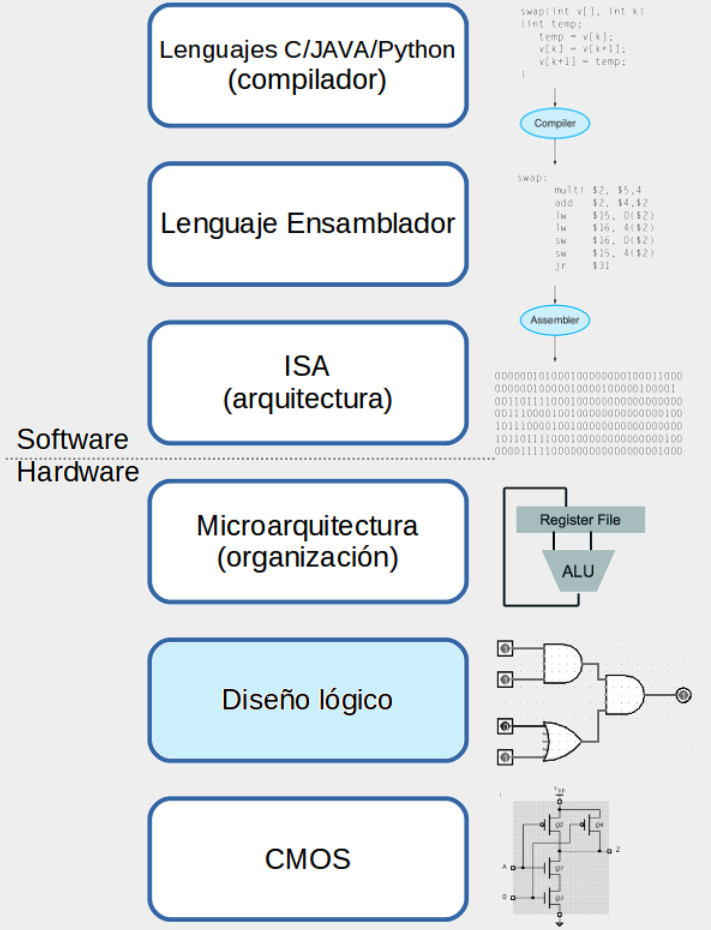
\includegraphics[scale=0.2]{images/abstraccion-logico.jpg} 

    \end{columns}
\end{frame}


\subsection{Algebra de Boole}

\begin{frame}{Análisis de Circuitos Digitales}{Diseño lógico o digital}

\bigskip

 \begin{columns}[onlytextwidth,T]
      \column{\dimexpr\linewidth-60mm-5mm}

Orígenes de la teoría de análisis y diseño de circuitos lógicos
o digitales:
\begin{itemize}
\item[Booleano] En 1854 George Boole define un algebra que utiliza sólo dos valores.
\item[Switching] En 1938 Claude Shannon demuestra que el algebra de boole puede ser utilizado para analizar y modelar circuitos digitales.
\end{itemize}

\bigskip
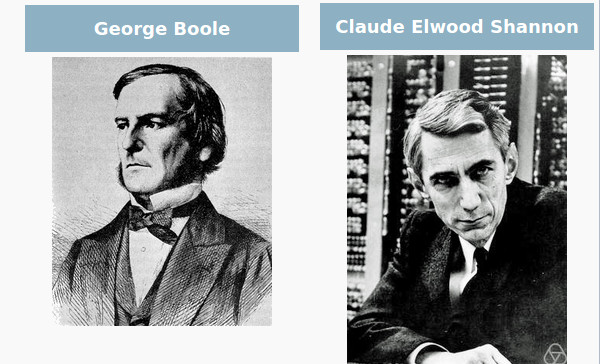
\includegraphics[scale=0.3]{images/boole-shannon.jpg} 
      \column{60mm}
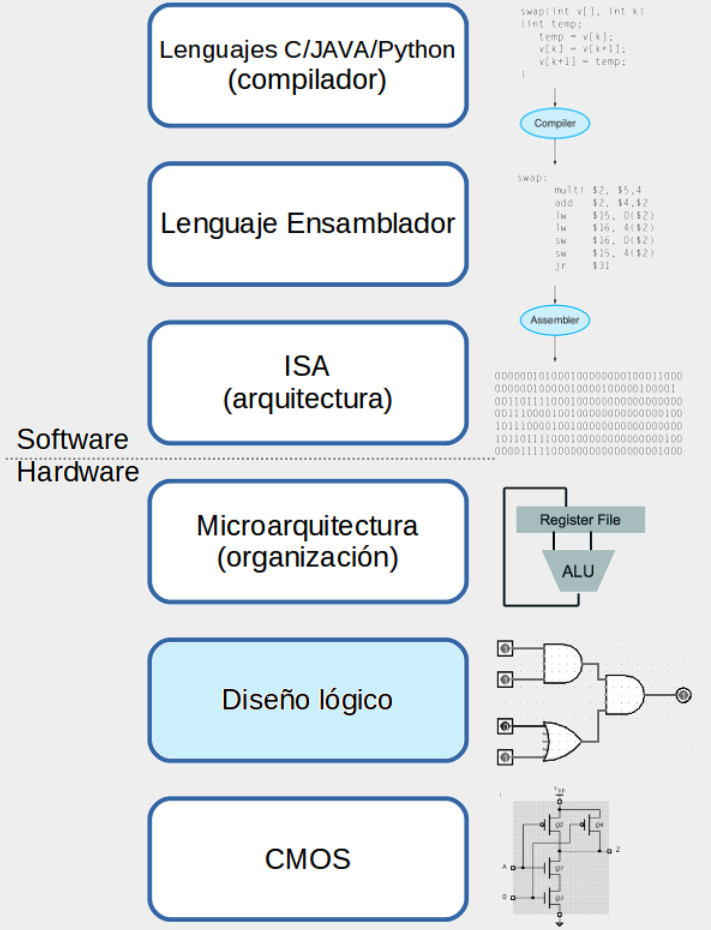
\includegraphics[scale=0.2]{images/abstraccion-logico.jpg} 

    \end{columns}
\end{frame}




\begin{frame} {Circuitos Combinacionales} {Compuertas, Tablas de Verdad, Ecuaciones Lógicas}
\bigskip
\textbf{Circuito combinacional:} La función lógica (salida) depende únicamente de las señales de entrada.
\bigskip
\begin{center}\textbf{Tablas de Verdad}\end{center}
\begin{itemize}
\item Debido a que un bloque de lógica combinatoria 
no contiene memoria, puede especificarse 
completamente definiendo los valores de las 
salidas para cada posible conjunto de valores 
de entrada
\item 
Dicha descripción se da normalmente en forma 
de 
tabla de verdad

\end{itemize}
\end{frame}




\begin{frame} {Circuitos Combinacionales} {Compuertas, Tablas de Verdad, Ecuaciones Lógicas}
\begin{center}\textbf{Tablas de Verdad}\end{center}
\begin{itemize}
\item Para un bloque lógico con n entradas, existen   2 n posiciones en la tabla de verdad, puesto que 
este es el número de combinaciones posible de 
los valores de entrada
\item Cada posición en la tabla especifica el valor de 
todas las salidas para una combinación 
particular de las entrada
\item Las tablas de verdad pueden \textbf{describir 
completamente cualquier función lógica} 
combinatoria
\item Sin embargo, su tamaño \textbf{crece rápidamente} y 
puede dificultar su comprensión

\end{itemize}
\end{frame}


%\begin{frame}
%\frametitle{Compuertas, Tablas de Verdad, Ecuaciones Lógicas}
%\begin{center}\textbf{Tablas de Verdad}\end{center}
%\begin{figure}
%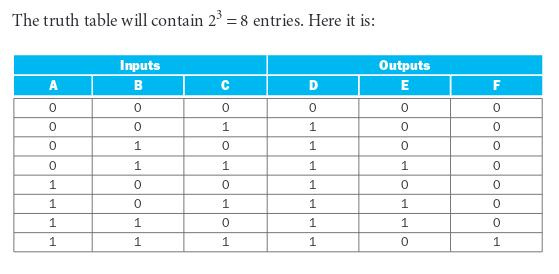
\includegraphics[scale=0.4]{tabla.jpg} 
%\end{figure}
%
%
%\end{frame}











\begin{frame} {Circuitos Combinacionales} {Compuertas, Tablas de Verdad, Ecuaciones Lógicas}
\begin{center}\textbf{Algebra de Boole}\end{center}
\begin{itemize}
\item Todas la variable tienen valores 0 ó 1
\item Existen tres operadores:
\begin{itemize}
\item \textbf{OR}
, se escribe 
+
, como en 
A +B
. El resultado es 1 si alguna 
de la variables de entrada es 1. También se conoce como 
suma lógica
\item \textbf{AND}
, se escribe
 .
, como en
 A.B
. El resultado es 1 sólo si 
ambas entradas son 1. También se conoce como 
producto 
lógico
\item \textbf{NOT}
, se escribe      . El resultado es 1 sólo si la entrada es 0. 
La aplicación del operador NOT a un valor lógico resulta en 
una inversión o negación de dicho valor 
\end{itemize}
\end{itemize}
\end{frame}






\begin{frame} {Circuitos Combinacionales} {Compuertas, Tablas de Verdad, Ecuaciones Lógicas}
\begin{center}\textbf{Álgebra de Boole - Leyes y Teoremas}\end{center}
\begin{figure}
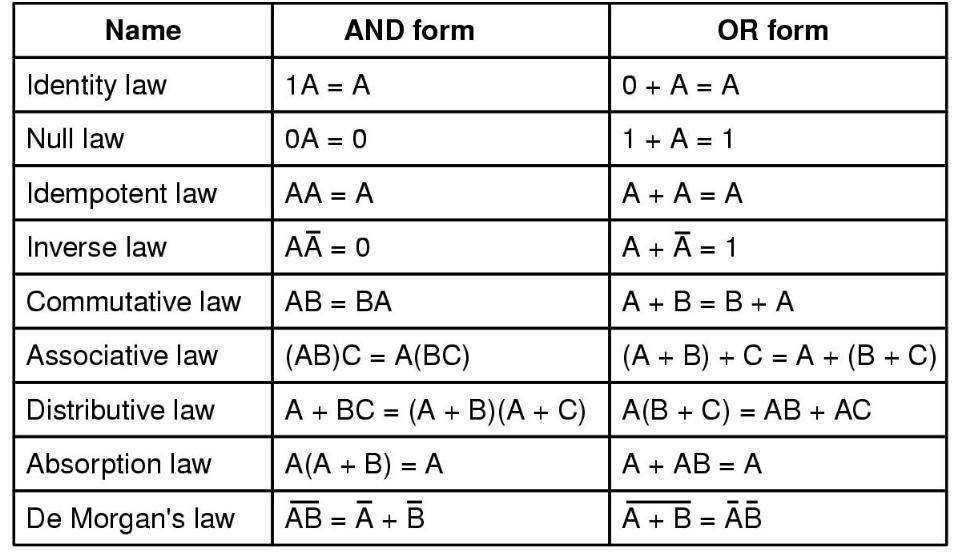
\includegraphics[scale=0.2]{images/leyes.jpg} 
\end{figure}
\end{frame}







\begin{frame} {Circuitos Combinacionales} {Compuertas, Tablas de Verdad, Ecuaciones Lógicas}
\begin{center}\textbf{Álgebra de Boole - Leyes y Teoremas}\end{center}
\begin{itemize}
\item Cualquier función lógica puede ser reescrita como una ecuación, 
con la salida en la parte izquierda de la igualdad, y una función 
de las variables de entrada utilizando las operaciones del álgebra a la derecha.

\item Ejemplo:
\end{itemize}
\begin{figure}
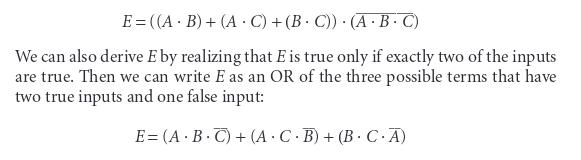
\includegraphics[scale=0.4]{images/ecuacion.jpg} 
\end{figure}
\end{frame}




\begin{frame} {Circuitos Combinacionales} {Compuertas, Tablas de Verdad, Ecuaciones Lógicas}
\begin{center}\textbf{Compuertas/Puertas (Gates)}\end{center}
\begin{itemize}
\item Los bloques lógicos se construyen a partir de 
compuertas (puertas) lógicas
 que realizan las 
funciones lógicas básicas como AND, OR y NOT
\item Una puerta AND o una OR pueden tener 
múltiples entradas, con la salida igual a la AND o 
la OR de todas ellas
\item La función lógica NOT se realiza mediante un 
inversor que siempre tiene una entrada
\end{itemize}

\end{frame}





\begin{frame} {Circuitos Combinacionales} {Compuertas, Tablas de Verdad, Ecuaciones Lógicas}
\begin{center}\textbf{Compuertas/Puertas (Gates)}\end{center}
\begin{figure}
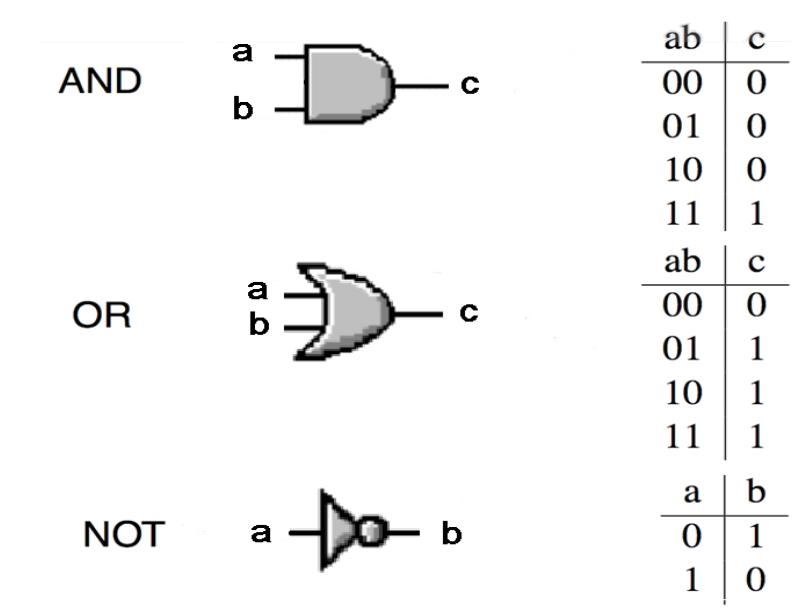
\includegraphics[scale=0.2]{images/compuertas.jpg} 
\end{figure}
\end{frame}


\begin{frame} {Circuitos Combinacionales} {Compuertas, Tablas de Verdad, Ecuaciones Lógicas}
\begin{center}\textbf{Compuertas/Puertas (Gates)}\end{center}
\begin{figure}
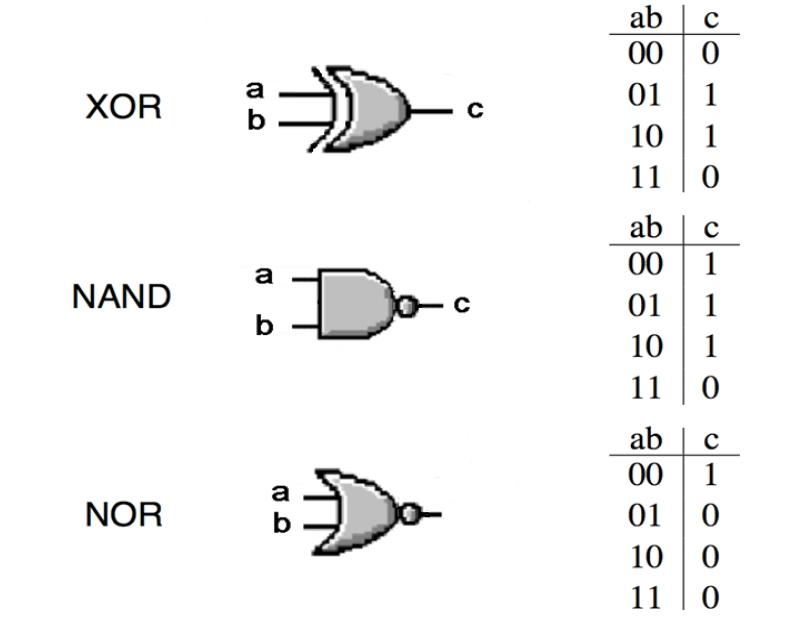
\includegraphics[scale=0.2]{images/compuertasx.jpg} 
\end{figure}
\end{frame}

\subsection{Metodología para realizar un diseño lógico/digital}

\begin{frame} {Circuitos Combinacionales} {Diseño digital}

 \begin{columns}[onlytextwidth,T]
      \column{\dimexpr\linewidth-60mm-5mm}
\textbf{Metodología para realizar un diseño lógico/digital de un circuito combinacional}
\bigskip
\begin{enumerate}
\item Definir coloquialmente todas las entradas y todas las salidas
\item Confeccionar una tabla de verdad para todas las combinaciones de valores de entrada y todas las salidas
\item Describir para cada salida una función lógica en base a la tabla
\item Confeccionar un diagrama del circuito digital resultante
\end{enumerate}

	\column{60mm}

\begin{figure}
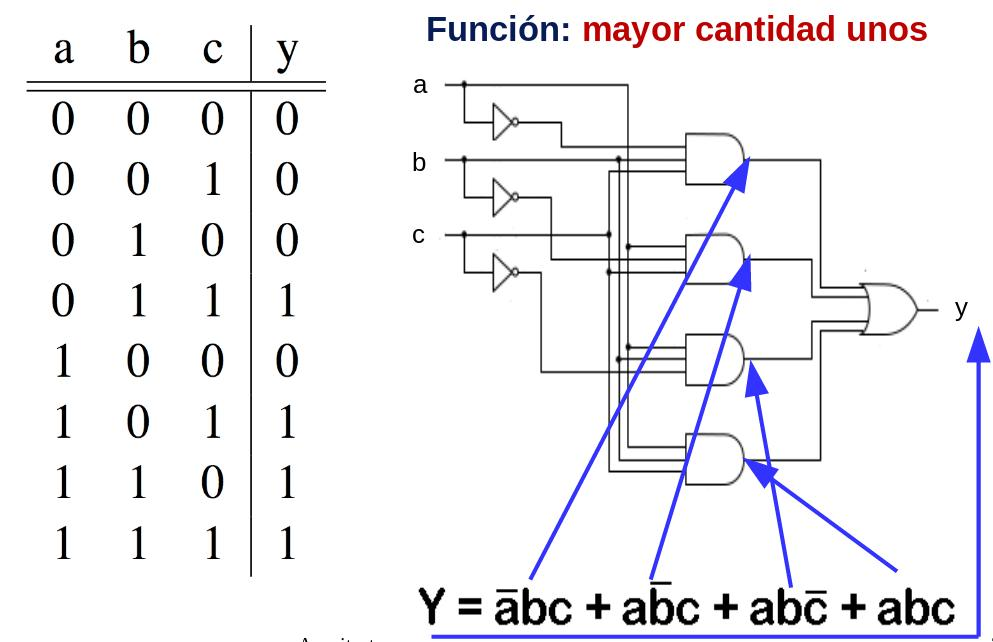
\includegraphics[scale=0.18]{images/construcciondigital.jpg} 
\end{figure}
  \end{columns}
\end{frame}


\subsection{Circuitos combinacionales comunes}


\begin{frame} {Circuitos Combinacionales} {Diseño digital}
\begin{center}\textbf{Construcción de diseño lógico/digital: Decoder}\end{center}
\begin{figure}
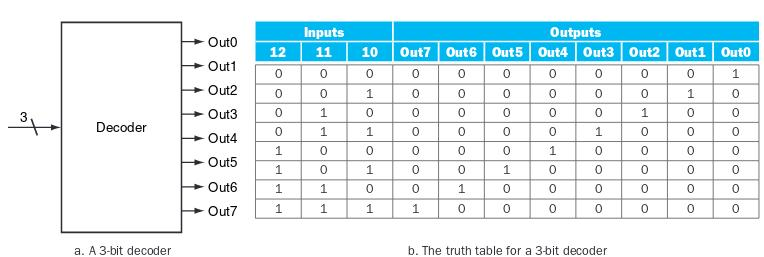
\includegraphics[scale=0.4]{images/decoder.jpg} 
\end{figure}
\end{frame}


\begin{frame} {Circuitos Combinacionales} {Diseño digital}
\begin{center}\textbf{Construcción de diseño lógico/digital: Multiplexor}\end{center}
\begin{figure}
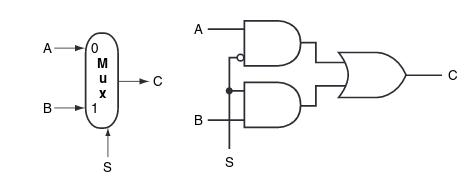
\includegraphics[scale=0.4]{images/multiplexor.jpg} 
\end{figure}
\end{frame}



\begin{frame} {Circuitos Combinacionales} {Diseño digital}
\begin{center}\textbf{Construcción de diseño lógico/digital: Multiplexor 32 bits}\end{center}
\begin{figure}
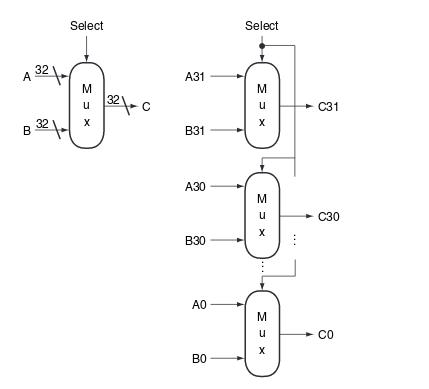
\includegraphics[scale=0.4]{images/multiplexor32bits.jpg} 
\end{figure}
\end{frame}




\begin{frame} {Circuitos Combinacionales} {Diseño digital}
\begin{center}\textbf{Diseño de ALU de un bit}\end{center}
\begin{figure}
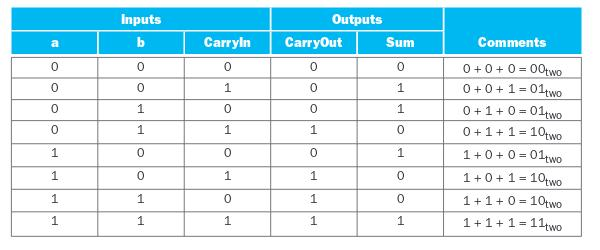
\includegraphics[scale=0.4]{images/alu1bit.jpg} 
\end{figure}
\end{frame}




\begin{frame} {Circuitos Combinacionales} {Diseño digital}
\begin{center}\textbf{Diseño de ALU de un bit}\end{center}
\begin{figure}
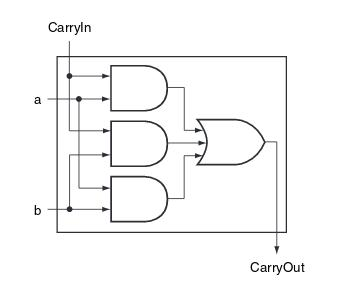
\includegraphics[scale=0.4]{images/alu1bit-2.jpg} 
\end{figure}
\end{frame}




\begin{frame} {Circuitos Combinacionales} {Diseño digital}
\begin{center}\textbf{Diseño de ALU de un bit}\end{center}
\begin{figure}
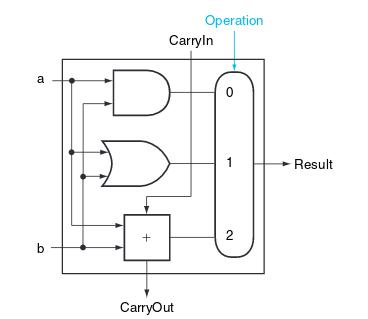
\includegraphics[scale=0.4]{images/alu1bit-3.jpg} 
\end{figure}
\end{frame}


\begin{frame} {Circuitos Combinacionales} {Diseño digital}
\begin{center}\textbf{Diseño de ALU de un bit}\end{center}
\begin{figure}
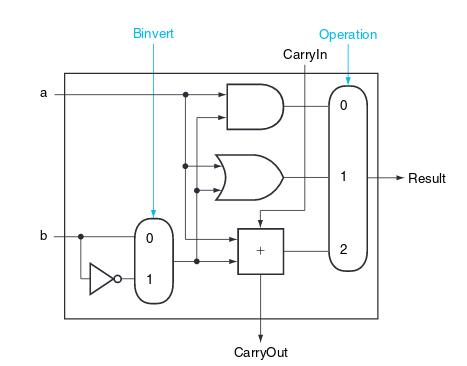
\includegraphics[scale=0.4]{images/alu1bit-4.jpg} 
\end{figure}
\end{frame}


\begin{frame} {Circuitos Combinacionales} {Diseño digital}
\begin{center}\textbf{Diseño de ALU de 32 bits}\end{center}
\begin{figure}
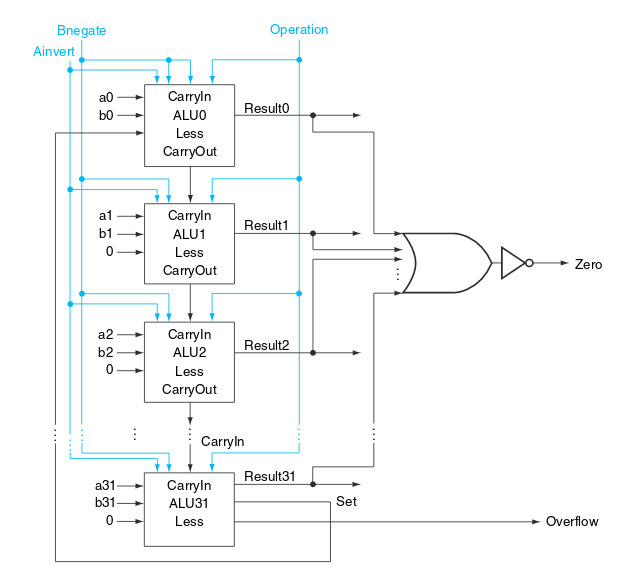
\includegraphics[scale=0.4]{images/alu1bit-5.jpg} 
\end{figure}
\end{frame}


\begin{frame} {Circuitos Combinacionales} {Diseño digital}
\begin{center}\textbf{Diseño de una unidad de control}\end{center}
\begin{figure}
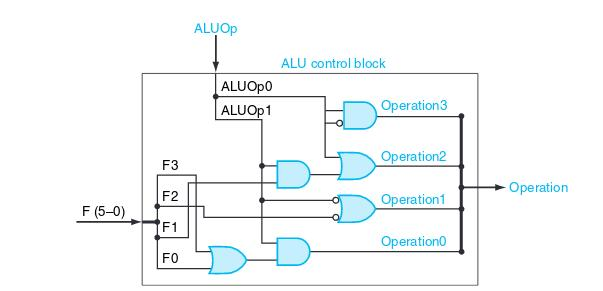
\includegraphics[scale=0.4]{images/control.jpg} 
\end{figure}
\end{frame}


\subsection{Relojes}

\begin{frame}{Relojes}{Diseño digital}
\begin{center}\textbf{Relojes}\end{center}
\begin{itemize}
\item Los relojes son necesarios en la lógica secuencial, para decidir cuando un elemento que contiene un estado debe ser actualizado.
\item Terminología: tiempo del ciclo (período), frecuencia del reloj.
\item Metodología : edge-triggered clocking (reloj disparado por flanco)
\end{itemize}
\begin{figure}
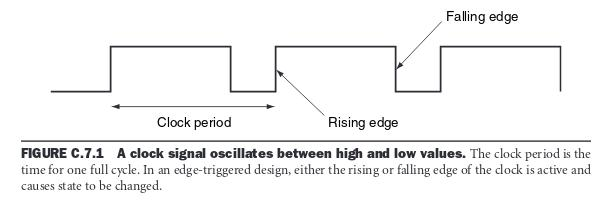
\includegraphics[scale=0.4]{images/reloj.jpg} 
\end{figure}
\end{frame}


\begin{frame}{Relojes}{Diseño digital}
\begin{center}\textbf{Relojes}\end{center}
\begin{itemize}
\item Sistemas síncronos
\item edge-triggered clocking posibilita un proceso instantáneo
\end{itemize}
\begin{figure}
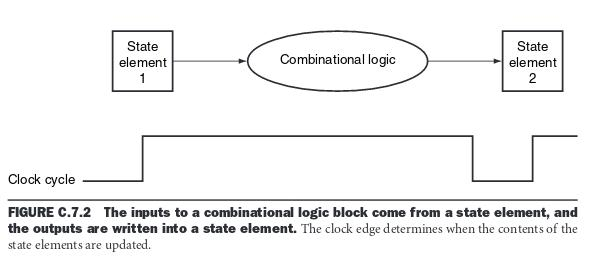
\includegraphics[scale=0.4]{images/reloj-estado-combinacional.jpg} 
\end{figure}
\end{frame}


\subsection{Circuitos secuenciales}

\begin{frame}{Circuitos secuenciales}{Diseño digital}
\bigskip
\textbf{Elementos de memoria: Set-Reset Latch}
\begin{itemize}
\item Elemento básico para almacenar un bit. Contiene un Loop en su diseño.
\end{itemize}
\bigskip
\begin{figure}
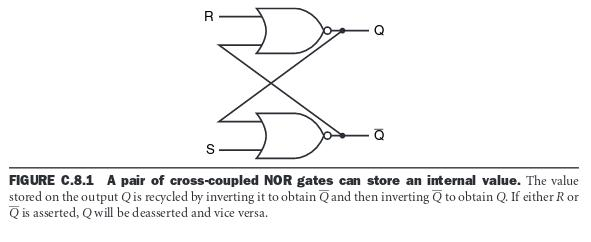
\includegraphics[scale=0.4]{images/latch-s-r.jpg} 
\end{figure}
\end{frame}

\begin{frame}{Circuitos secuenciales}{Diseño digital}
\bigskip
\textbf{Elementos de memoria: D Latch}
\begin{itemize}
\item Elemento básico para almacenar un bit. Contiene un Loop en su diseño
\item Sus entradas son el bit a almacenar y la señal de reloj
\end{itemize}
\bigskip
\begin{figure}
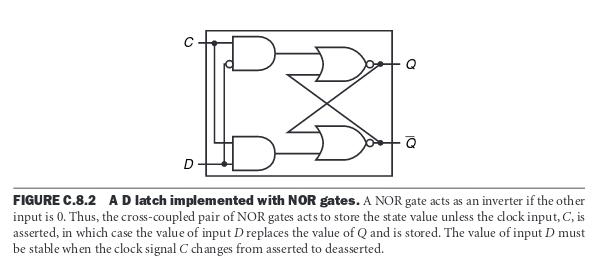
\includegraphics[scale=0.4]{images/latch-d.jpg} 
\end{figure}
\end{frame}


\begin{frame}{Circuitos secuenciales}{Diseño digital}
\bigskip
\textbf{Elementos de memoria: D Latch}
\bigskip
\begin{figure}
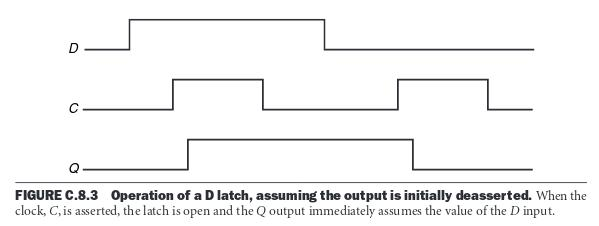
\includegraphics[scale=0.4]{images/latch-d-tiempo.jpg} 
\end{figure}
\end{frame}


\begin{frame}{Circuitos secuenciales}{Diseño digital}
\bigskip
\textbf{Elementos de memoria: D Flip-Flop}
\begin{itemize}
\item D Flip-Flop : utilizados en la construcción de REGISTROS
\item Elemento básico para almacenar un bit. Contiene un Loop en su diseño
\item Sus entradas son el bit a almacenar y la señal de reloj
\item Se sincroniza (actualiza) en el flanco de reloj
\end{itemize}
\bigskip
\begin{figure}
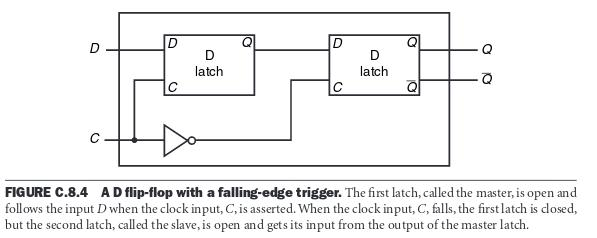
\includegraphics[scale=0.4]{images/flip-flop-d.jpg} 
\end{figure}
\end{frame}

\begin{frame}{Circuitos secuenciales}{Diseño digital}
\bigskip
\textbf{Elementos de memoria: D Flip-Flop}
\begin{itemize}
\item Si la señal D cambia cuando la señal de reloj está baja (desacertada)
el estado interno del flip-flop no cambia. Eso lo distingue de un latch.
\end{itemize}
\bigskip
\begin{figure}
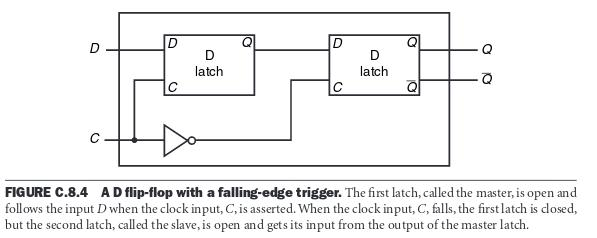
\includegraphics[scale=0.4]{images/flip-flop-d.jpg} 

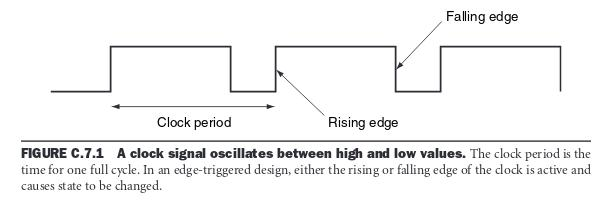
\includegraphics[scale=0.4]{images/reloj.jpg} 
\end{figure}
\end{frame}

\begin{frame}[fragile]
\frametitle{Diseño digital}
\begin{center}\textbf{Diseño de ALU y Registros}\end{center}
\begin{itemize}
\item Elementos de estado, multiplexores, decodificadores, ALU
\end{itemize}
\begin{figure}
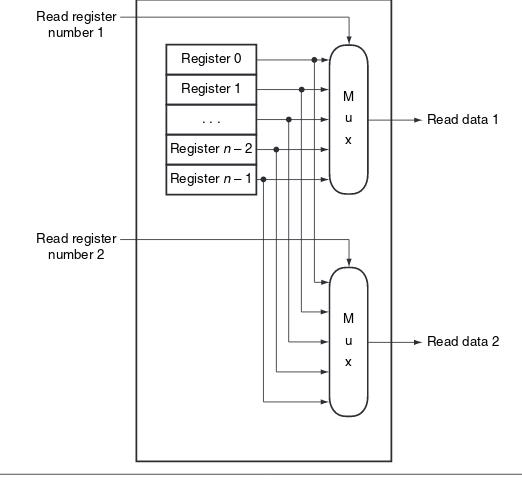
\includegraphics[scale=0.4]{images/leer-registro.jpg} 
\end{figure}
\end{frame}

\begin{frame}[fragile]
\frametitle{Diseño digital}
\begin{center}\textbf{Diseño de ALU y Registros}\end{center}
\begin{itemize}
\item Elementos de estado, multiplexores, decodificadores, ALU
\end{itemize}
\begin{figure}
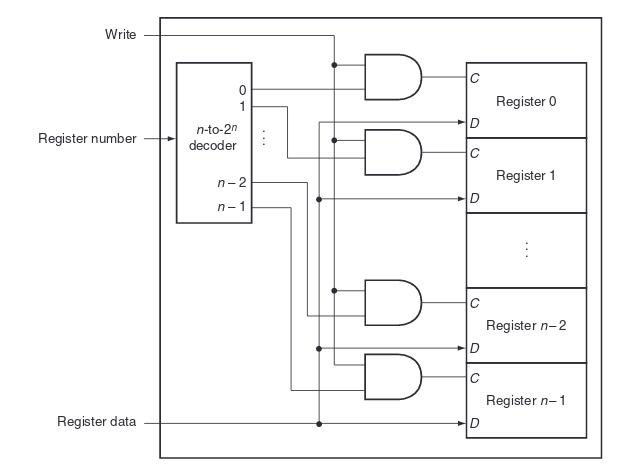
\includegraphics[scale=0.4]{images/escribir-registro.jpg} 
\end{figure}
\end{frame}


\subsection{Máquinas de Estado Finito (FSM)}


\begin{frame}[fragile]
\frametitle{Diseño digital}
\begin{center}\textbf{Máquinas de Estado Finito (FSM)}\end{center}
\begin{itemize}
\item Permiten especificar circuitos secuenciales
\item Ejemplo: control de la calefacción de un coche
\end{itemize}
\begin{figure}
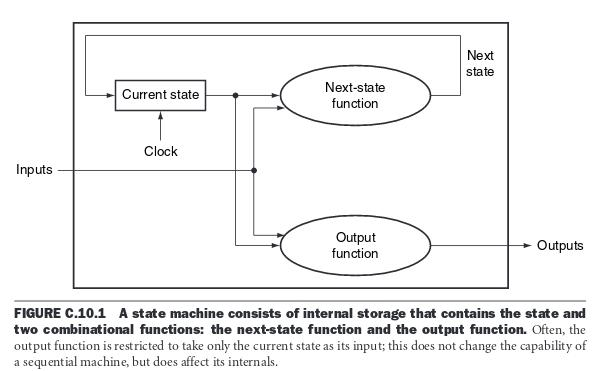
\includegraphics[scale=0.4]{images/fsm1.jpg} 
\end{figure}
\end{frame}


\begin{frame}[fragile]
\frametitle{Diseño digital}
\begin{center}\textbf{Máquinas de Estado Finito (FSM)}\end{center}
Existen dos clasificaciones teóricas:
\begin{itemize}
\item Autómata de Mealy
\item Autómata de Moore
\end{itemize}
\begin{figure}
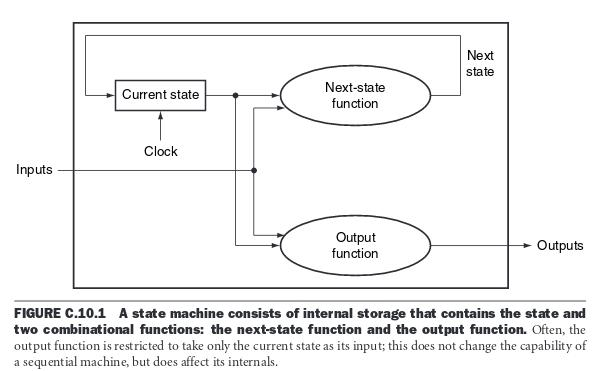
\includegraphics[scale=0.4]{images/fsm1.jpg} 
\end{figure}
\end{frame}



\begin{frame}[fragile]
\frametitle{Diseño digital}
\begin{center}\textbf{Máquinas de Estado Finito (FSM)}\end{center}
\begin{itemize}
\item Ejemplo: Luces de giro del Ford Thunderbird
\end{itemize}
\begin{figure}
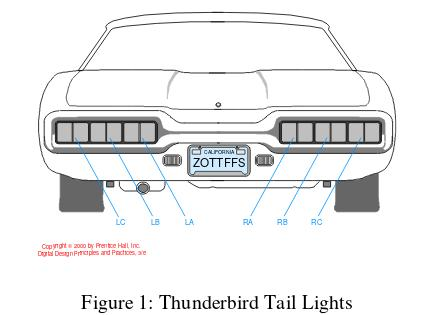
\includegraphics[scale=0.4]{images/fsm2.jpg} 
\end{figure}
\end{frame}

\begin{frame}[fragile]
\frametitle{Diseño digital}
\begin{center}\textbf{Máquinas de Estado Finito (FSM)}\end{center}
\begin{itemize}
\item Ejemplo: Luces de giro del Ford Thunderbird
\end{itemize}
\begin{figure}
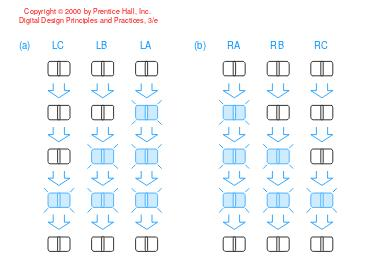
\includegraphics[scale=0.4]{images/fsm3.jpg} 
\end{figure}
\end{frame}

\begin{frame}[fragile]
\frametitle{Diseño digital}
\begin{center}\textbf{Máquinas de Estado Finito (FSM)}\end{center}
\begin{itemize}
\item Ejemplo: Luces de giro del Ford Thunderbird
\item Diagrama de estados
\end{itemize}
\begin{figure}
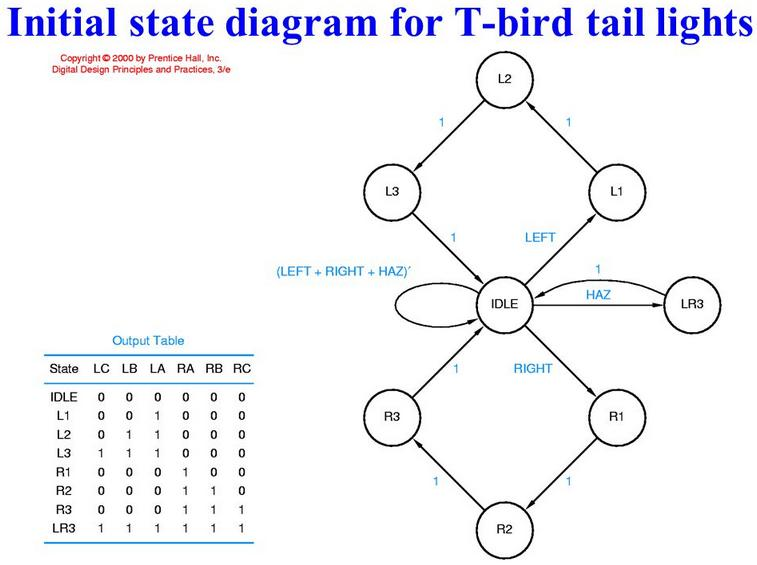
\includegraphics[scale=0.25]{images/fsm4.jpg} 
\end{figure}
\end{frame}

\begin{frame}[fragile]
\frametitle{Diseño digital}
\begin{center}\textbf{Máquinas de Estado Finito (FSM)}\end{center}
\begin{itemize}
\item Ejemplo: Luces de giro del Ford Thunderbird
\item Diagrama de estados (segunda versión)
\end{itemize}
\begin{figure}
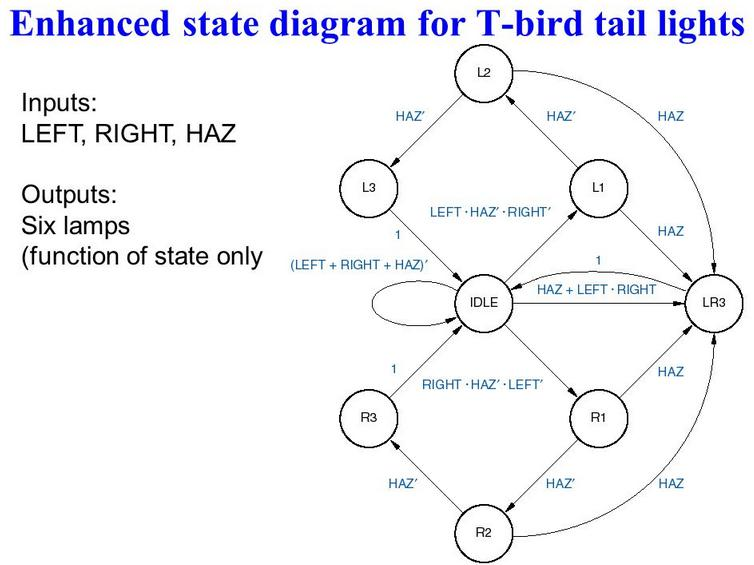
\includegraphics[scale=0.25]{images/fsm5.jpg} 
\end{figure}
\end{frame}

\begin{frame}{Sistema de climatización digital}{Máquinas de Estado Finito (FSM)}
\begin{columns}[onlytextwidth,T]
\column{\dimexpr\linewidth-60mm-5mm}
\bigskip
\bigskip
\begin{itemize}
\item El sistema cuenta con tres entradas: 
\begin{itemize}
\item pulsador Up (subir temperatura)
\item pulsador Down (bajar temperatura)
\item termostato
\end{itemize}
\item La salida es el control de temperatura y el display
\bigskip
\item Una implementación es a través de 5 estados: mín. temp., frío, templado, caluroso, max. temp.
\end{itemize}
       \column{60mm}
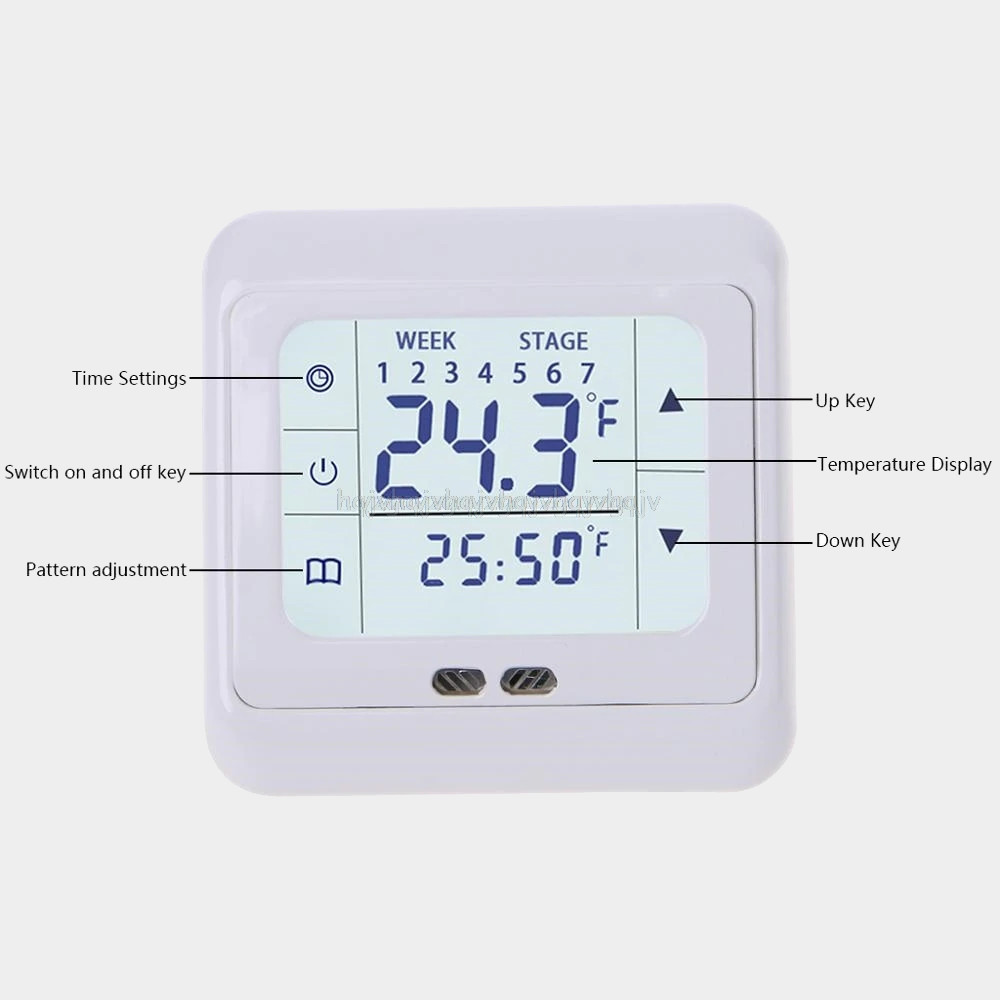
\includegraphics[scale=0.2]{images/temp.jpg} 
    \end{columns}
\end{frame}





\begin{frame}{Máquina Algorítmica de Multiplicación}
\begin{columns}[onlytextwidth,T]
\column{\dimexpr\linewidth-70mm-5mm}
\bigskip
\bigskip

\begin{footnotesize}
\begin{itemize}
\item Implementa un algoritmos de multiplicación en hardware
\item Control en este caso es una máquina de estado finito
\begin{footnotesize}
\begin{itemize}
\item Contiene memoria (registro) para conocer en qué etapa de la multipiclación se encuentra
\bigskip
\item Si write y shift se hacen en ciclos de reloj distintos, entonces existen dos estados en cada iteración de la multiplicación
\end{itemize}
\end{footnotesize}
\bigskip
\end{itemize}
\end{footnotesize}

       \column{60mm}
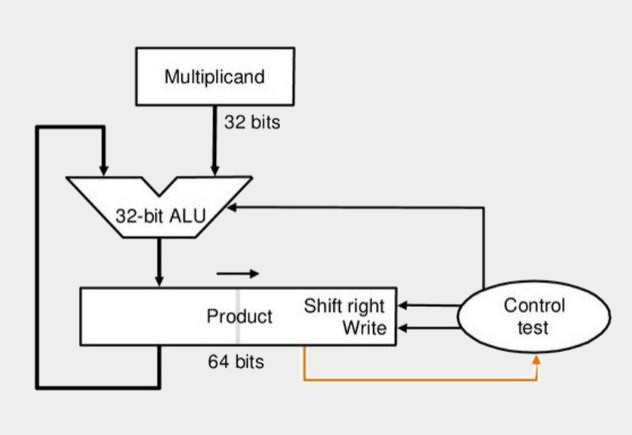
\includegraphics[scale=0.25]{images/maq-alg-mult.jpg} 

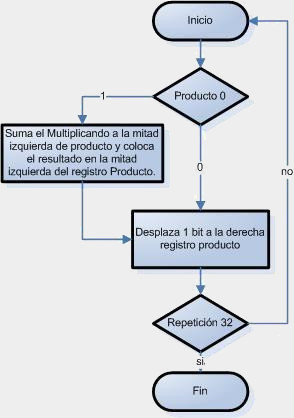
\includegraphics[scale=0.25]{images/alg.jpg} 
    \end{columns}
\end{frame}



\begin{frame}{Máquina Algorítmica de Multiplicación}
\begin{columns}[onlytextwidth,T]
\column{\dimexpr\linewidth-70mm-5mm}
\bigskip
\bigskip

\begin{footnotesize}
\begin{itemize}
\item Implementa un algoritmos de multiplicación en hardware
\item Tarea:
\begin{footnotesize}
\begin{itemize}
\item Multiplicar dos números de 4 bits utilizando la máquina algorítmica descripta.
\bigskip
\item Por ejemplo: 3 (0011) x 5 (0101)
\bigskip
\item Entender el funcionamiento de la máquina verificando los resultados parciales de las sumas del registro producto.
\end{itemize}
\end{footnotesize}
\bigskip
\end{itemize}
\end{footnotesize}

       \column{60mm}
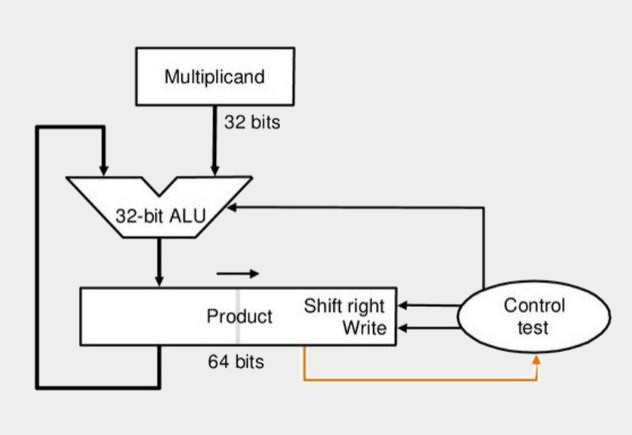
\includegraphics[scale=0.25]{images/maq-alg-mult.jpg} 

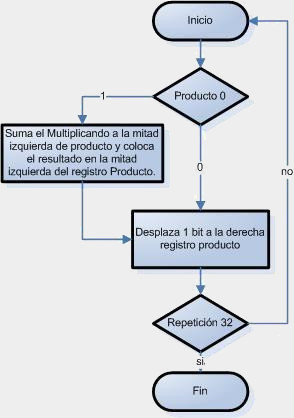
\includegraphics[scale=0.25]{images/alg.jpg} 
    \end{columns}
\end{frame}


\begin{frame}
 \frametitle{Bibliografía}
Libros
\begin{itemize}
\item Apunte Diseño Lógico (disponible en la web de la materia)
\item David. Patterson John L. Hennessy (1995), ORGANIZACIÓN Y DISEÑO DE COMPUTADORES La interfaz hardware/software, McGraw-Hill (8 copias en biblioteca).
\end{itemize}
\end{frame}


\end{footnotesize}

\end{document}





